% ATKINSON, P. (2008). A bitter pill to swallow: the rise and fall of the tablet computer.
% Design issues, 24 (4), 3-25. [Article]
% Davis, M., Ellis, T. (1964). The RAND Tablet: A man-machine graphical communication device.
% The RAND Corporation.
\begin{frame}
\frametitle{1964 - The RAND Tablet}
\begin{columns}
    \begin{column}{0.45\textwidth}
        \centering
        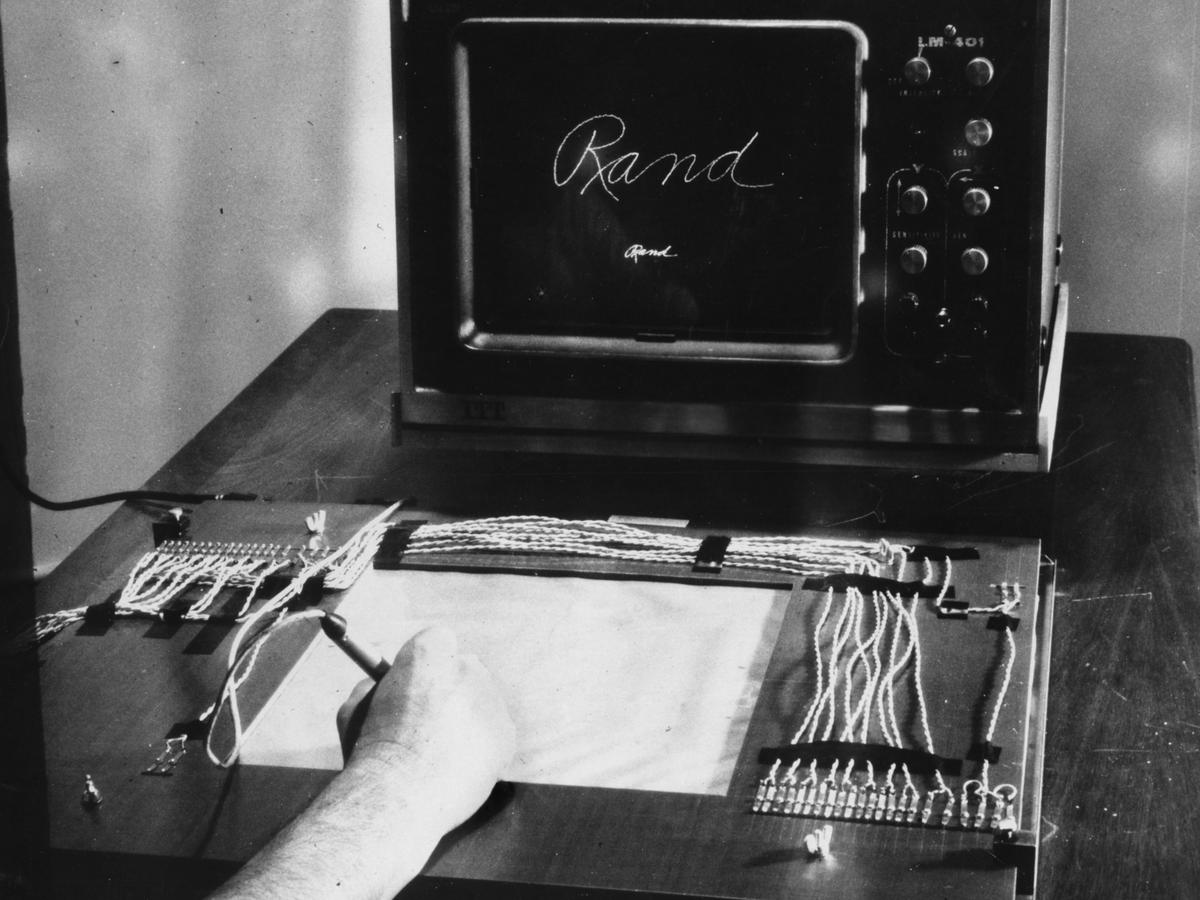
\includegraphics[width=\linewidth]{assets/rand-tablet.jpeg}
    \end{column}

    \begin{column}{0.45\textwidth}
        The RAND Corportation created the RAND tablet, also known as the Grafacon, a device intended for handwriting recognition via stylus. It was apparently the first graphic device that was: digital, low-cost, able to describe 10^6 locations on the screen, and had good linearity.
    \end{column}
\end{columns}
\end{frame}
%==================================================================================
% https://www.columbia.edu/cu/computinghistory/2250.html
\begin{frame}
\frametitle{1964 - The IBM 2250}
\begin{columns}
    \begin{column}{0.45\textwidth}
        \centering
        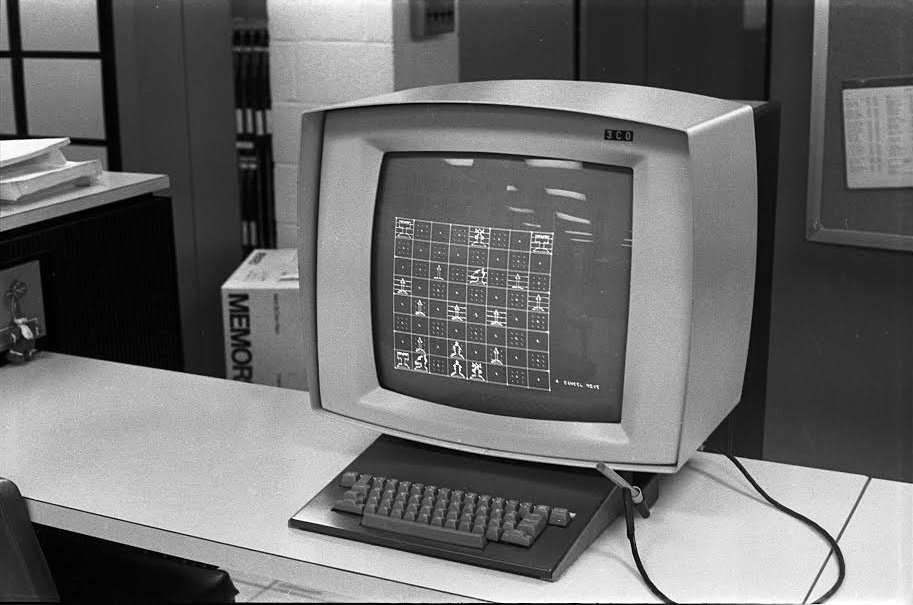
\includegraphics[width=\linewidth]{assets/ibm-2250.jpg}
    \end{column}

    \begin{column}{0.45\textwidth}
        The IBM 2250 Graphics Display Unit was announced. It was made to display and interact with cloud chamber images. At the time, an entire system would cost approximately $280 000.
    \end{column}
\end{columns}
\end{frame}